\chapter{Introduzione}
La cosmologia studia la composizione, la struttura su grande scala e l'evoluzione dell'Universo. Il quadro attuale si basa sul confronto tra modelli teorici e osservazioni indipendenti, che indicano un Universo in espansione, originato da una fase molto calda e densa, e dominato oggi da componenti la cui natura fisica rimane in gran parte sconosciuta. Nel modello cosmologico standard, circa il $5\%$ del contenuto energetico attuale è costituito da materia ordinaria, o barionica, presente nelle stelle, nei pianeti e soprattutto nel gas diffuso. Circa il $27\%$ è attribuito alla \emph{materia oscura} e il restante $68\%$ all'\emph{energia oscura}. Queste percentuali si riferiscono alla densità totale di materia ed energia, non alla sola materia. La materia oscura manifesta la propria presenza attraverso gli effetti gravitazionali, senza emettere o assorbire luce in misura apprezzabile; l'energia oscura è invece la componente introdotta per spiegare l'espansione accelerata dell'Universo.

Una delle principali evidenze della materia oscura proviene dalle curve di rotazione delle galassie a spirale, studiate, tra gli altri, da Vera Rubin e dai suoi collaboratori. Nelle regioni esterne, la velocità orbitale di stelle e gas rimane approssimativamente costante, anziché diminuire come ci si attenderebbe oltre la regione contenente la maggior parte della massa visibile. Questo comportamento suggerisce la presenza di un alone esteso di materia non luminosa.

Lo studio dell'espansione cosmica si avvale anche delle supernove di tipo Ia, esplosioni termonucleari di nane bianche in sistemi binari. In uno degli scenari possibili, una nana bianca accresce materia da una compagna avvicinandosi alla massa di Chandrasekhar, circa $1.4\,M_\odot$, dove $M_\odot$ è la massa solare. Il confronto tra distanza e spostamento verso il rosso, o \emph{redshift}, ha fornito alla fine degli anni Novanta un'evidenza decisiva dell'accelerazione cosmica.

Un'altra osservazione fondamentale è la radiazione cosmica di fondo (\emph{Cosmic Microwave Background}, CMB), scoperta nel 1965. Essa è il residuo termico dell'Universo primordiale, divenuto trasparente alla luce circa $380.000$ anni dopo il Big Bang. Il suo spettro è estremamente vicino a quello di un corpo nero con temperatura attuale
\begin{equation}
    T_0 \simeq 2.725\,\mathrm{K}.
\end{equation}
La CMB è quasi uniforme, ma presenta piccole anisotropie, con fluttuazioni relative di temperatura dell'ordine di $\Delta T/T_0 \sim 10^{-5}$. Misurate dalle missioni COBE, WMAP e Planck con precisione crescente, queste anisotropie conservano informazioni sulle perturbazioni primordiali da cui si sono sviluppate le strutture cosmiche.

Il legame tra composizione e geometria dell'Universo è illustrato dai \emph{cosmic triangles}. Il parametro $\Omega_m$ comprende materia ordinaria e oscura, mentre $\Omega_\Lambda$ descrive l'energia oscura nell'ipotesi che sia una costante cosmologica $\Lambda$. Trascurando il piccolo contributo attuale della radiazione, l'equazione di Friedmann implica
\begin{equation}
    \Omega_m + \Omega_\Lambda + \Omega_k=1,
    \label{eq: somma contributi cosmici}
\end{equation}
dove $\Omega_k$ rappresenta il contributo della curvatura spaziale, non una componente materiale.
\begin{figure}[htbp]
    \centering
    \begin{subfigure}[t]{0.48\linewidth}
        \centering
        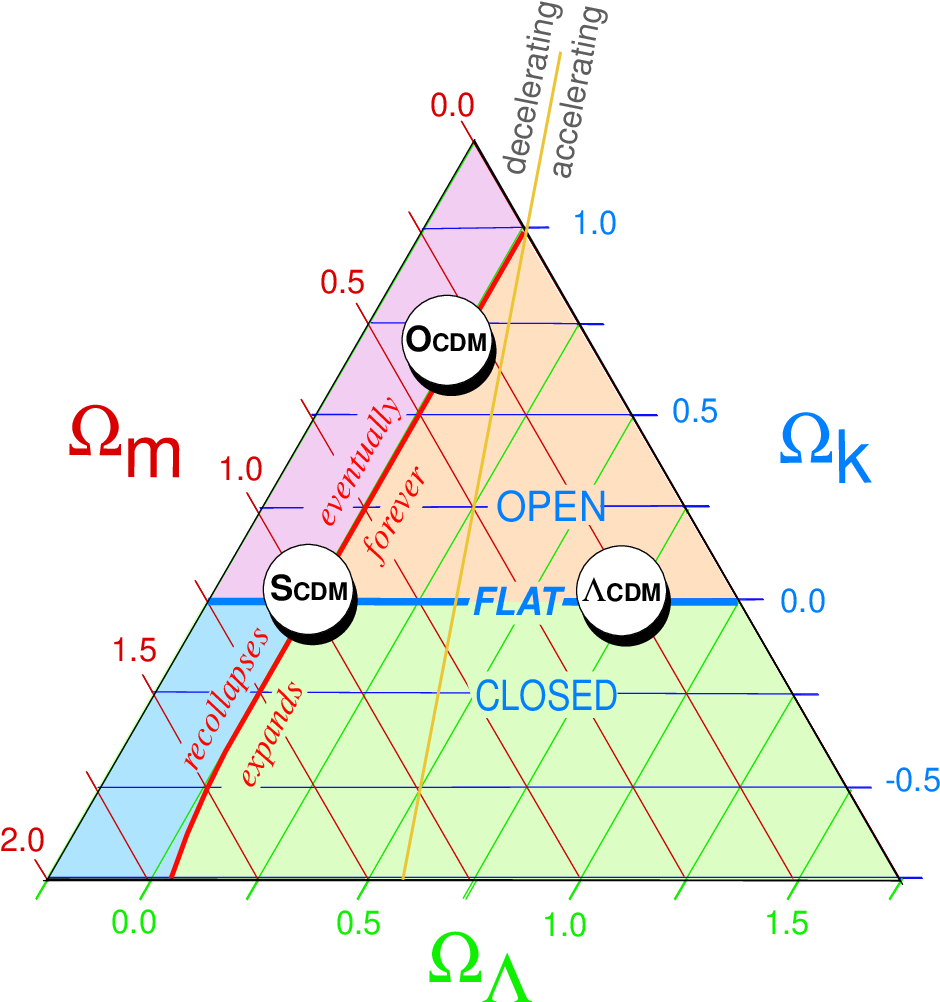
\includegraphics[width=\linewidth]{Immagini - Capitolo 1/Cosmic triangle 1.png}
        \caption{Cosmic triangle teorico con i modelli SCDM, OCDM e $\Lambda$CDM.}
        \label{fig: cosmic triangle teorico}
    \end{subfigure}\hfill
    \begin{subfigure}[t]{0.48\linewidth}
        \centering
        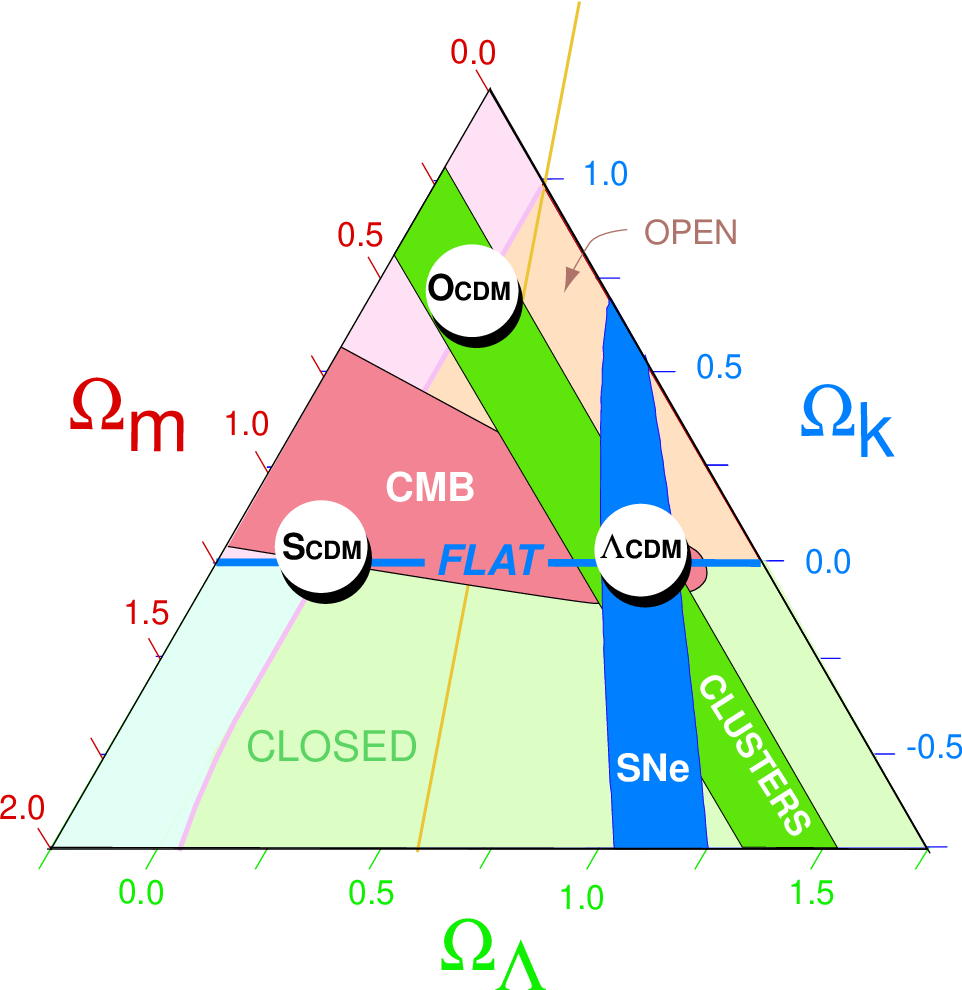
\includegraphics[width=\linewidth]{Immagini - Capitolo 1/Cosmic triangle 2.png}
        \caption{Cosmic triangle osservativo dove le misure convergono
        verso il modello $\Lambda$CDM.}
        \label{fig:cosmic triangle osservativo}
    \end{subfigure}
    \caption{Cosmic triangles.}
    \label{fig: cosmic triangles}
\end{figure}

Ogni punto dei diagrammi in figura \ref{fig: cosmic triangles} corrisponde alla terna di parametri $(\Omega_m,\Omega_\Lambda,\Omega_k)$ che soddisfa l'equazione \eqref{eq: somma contributi cosmici}; i valori si leggono seguendo le linee della griglia associate a ciascun parametro. Nella figura \ref{fig: cosmic triangle teorico}, la linea azzurra \emph{flat} identifica gli universi spazialmente piatti, con $\Omega_k = 0$. Le regioni \emph{open} e \emph{closed} corrispondono rispettivamente a $\Omega_k > 0$ a curvatura negativa e $\Omega_k < 0$ a curvatura positiva. La linea gialla separa l'espansione attualmente decelerata da quella accelerata. La linea rossa distingue invece i modelli che si espandono indefinitamente da quelli destinati a ricollassare, assumendo che $\Lambda$ rimanga costante. La geometria, quindi, non determina da sola il destino dell'Universo. Le sigle evidenziate confrontano tre modelli con materia oscura fredda (\emph{Cold Dark Matter}, CDM), cioè non relativistica durante la formazione delle strutture: SCDM indica il modello piatto con $\Omega_m = 1$ e $\Omega_\Lambda = 0$; OCDM un modello aperto con $\Omega_m < 1$ e $\Omega_\Lambda = 0$; $\Lambda$CDM un modello con materia oscura fredda e costante cosmologica, qui rappresentato nel caso piatto. 

In figura \ref{fig:cosmic triangle osservativo}, la fascia rosa mostra i vincoli della CMB, la fascia blu quelli delle supernove Ia (SNe) e la fascia verde quelli degli ammassi di galassie (\emph{clusters}). Queste osservazioni sondano rispettivamente soprattutto la geometria, la storia dell'espansione e la quantità di materia. La loro intersezione favorisce un Universo quasi piatto con $\Omega_m \simeq 0.3$ e $\Omega_\Lambda \simeq 0.7$.

Nel modello $\Lambda$CDM spazialmente piatto, fissate le ipotesi standard
su radiazione e neutrini, le proprietà statistiche delle anisotropie
della CMB si possono descrivere mediante sei parametri. Questi sono
\begin{equation}
    \{H_0,\Omega_m,\Omega_b,\tau,A_s,n_s\},
\end{equation}
dove:
\begin{enumerate}
    \item $H_0$ è la costante di Hubble legata al tasso di espansione dell'Universo;
    \item $\Omega_m$ è la densità complessiva di materia,
    ordinaria e oscura;
    \item $\Omega_b$ è la densità di materia barionica, per cui è una parte di $\Omega_m$;
    \item $\tau$ è la profondità ottica dovuta alla reionizzazione, 
    misura l'effetto della diffusione dei fotoni della CMB
    sugli elettroni liberi prodotti dalla successiva ionizzazione
    del gas cosmico;
    \item $A_s$ è l'ampiezza dello spettro delle perturbazioni
    primordiali di curvatura;
    \item $n_s$ è l'indice spettrale scalare, che descrive come tale
    spettro varia con la scala.
\end{enumerate}
La riduzione a sei parametri dipende comunque dalle ipotesi del modello. Se si consentisse, ad esempio, una curvatura non nulla o un'energia oscura
variabile nel tempo, occorrerebbero ulteriori parametri.